\documentclass[border=10pt]{standalone}
\usepackage{tikz}
\usepackage{xcolor}
\usetikzlibrary{arrows.meta,positioning,shapes.geometric,calc}

\definecolor{plan}{RGB}{70,130,180}
\definecolor{audit}{RGB}{60,160,100}
\definecolor{decide}{RGB}{210,120,40}
\definecolor{improve}{RGB}{160,60,120}
\definecolor{textgray}{RGB}{80,80,80}

\begin{document}
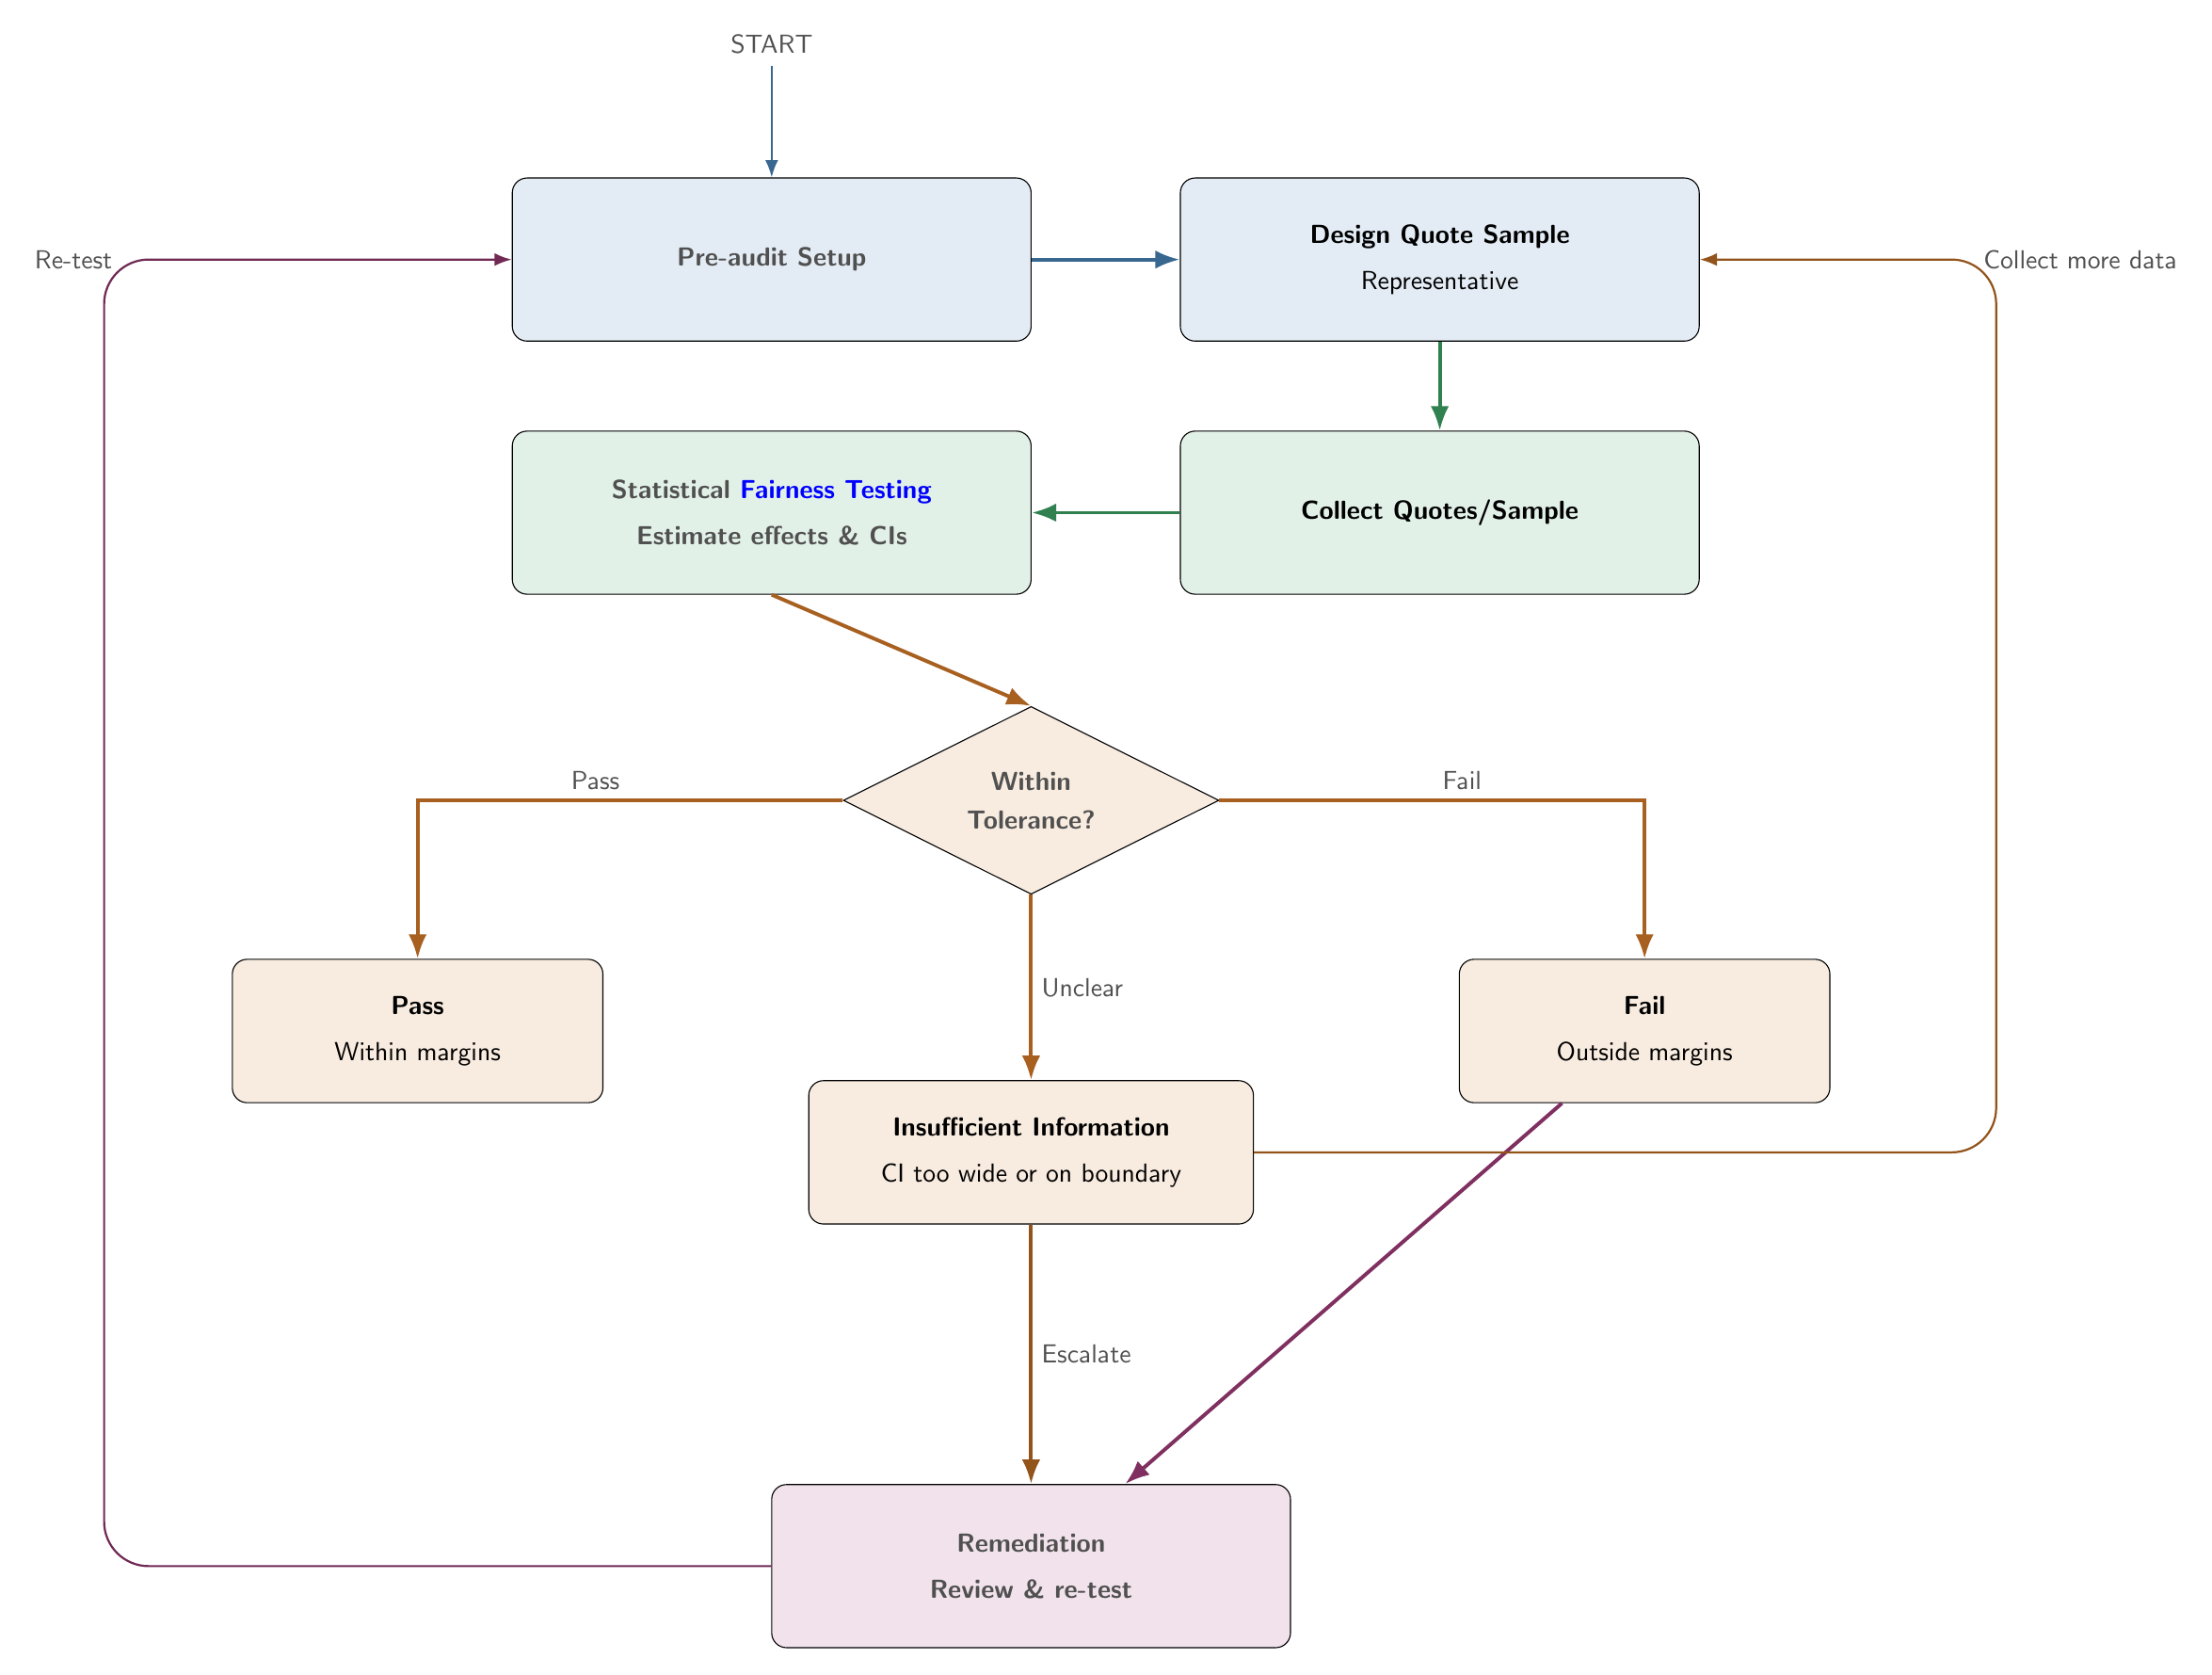
\begin{tikzpicture}[
  >=Latex,
  font=\sffamily,
  node distance=12mm and 20mm,
  box/.style={draw, rounded corners=2mm, align=center, inner sep=5mm,
    minimum width=70mm, minimum height=22mm, fill=white},
  decision/.style={draw, diamond, aspect=2, align=center,
    inner sep=3mm, fill=white},
  line/.style={-Latex, line width=.5mm},
  label/.style={font=\bfseries\sffamily, text=textgray},
  note/.style={font=\sffamily, text=textgray}
]
\node[box, fill=plan!15, label={[label, text=plan]above:PLAN}]
  (criterion) {\textbf{Pre-audit Setup}};
\node[box, fill=plan!15, right=of criterion] (design)
  {\textbf{Design Quote Sample}\\[2mm] Representative};
\node[box, fill=audit!15, below=of criterion,
  label={[label, text=audit]above:AUDIT}] (collect)
  {\textbf{Statistical \color{blue}{Fairness Testing}}\\[2mm]
   Estimate effects \& CIs};
\node[box, fill=audit!15, below=of design] (analyze)
  {\textbf{Collect Quotes/Sample}};
\node[decision, fill=decide!15, below=15mm of collect, xshift=35mm,
  label={[label, text=decide]above:DECIDE}] (equiv)
  {\textbf{Within}\\[1mm]\textbf{Tolerance?}};
\node[box, fill=decide!15, below left=15mm and 45mm of equiv,
  minimum width=50mm, minimum height=18mm] (pass)
  {\textbf{Pass}\\[2mm] Within margins};
\node[box, fill=decide!15, below=25mm of equiv,
  minimum width=60mm, minimum height=18mm] (insuff)
  {\textbf{Insufficient Information}\\[2mm] CI too wide or on boundary};
\node[box, fill=decide!15, below right=15mm and 45mm of equiv,
  minimum width=50mm, minimum height=18mm] (fail)
  {\textbf{Fail}\\[2mm] Outside margins};
\node[box, fill=improve!15, below=35mm of insuff,
  label={[label, text=improve]above:IMPROVE}] (remed)
  {\textbf{Remediation}\\[2mm] Review \& re-test};
\draw[-Latex, thick, color=plan!80!black]
  ([yshift=15mm]criterion.north) -- (criterion.north)
  node[midway, note, above=8mm of criterion]{START};
\draw[line, color=plan!80!black]   (criterion) -- (design);
\draw[line, color=audit!80!black]  (design) -- (analyze);
\draw[line, color=audit!80!black]  (analyze) -- (collect);
\draw[line, color=decide!80!black] (collect.south) -- (equiv.north);
\draw[line, color=decide!80!black] (equiv) -|
  node[near start, above left, note]{Pass} (pass);
\draw[line, color=decide!80!black] (equiv) --
  node[midway, right, note]{Unclear} (insuff);
\draw[line, color=decide!80!black] (equiv) -|
  node[near start, above right, note]{Fail} (fail);
\draw[line, color=improve!80!black] (fail) -- (remed);
\coordinate (rightboundary) at ([xshift=40mm]design.east);
\draw[-Latex, thick, color=decide!70!black, rounded corners=6mm]
  (insuff.east) -- (rightboundary |- insuff.east)
  -- (rightboundary |- design.east) -- (design.east)
  node[pos=0.75, right, note, xshift=27mm]{Collect more data};
\draw[line, color=decide!70!black]
  (insuff.south) -- (remed.north)
  node[midway, right, note]{Escalate};
\coordinate (leftboundary) at ([xshift=-55mm]criterion.west);
\draw[-Latex, thick, color=improve!70!black, rounded corners=6mm]
  (remed.west) -- (leftboundary |- remed.west)
  -- (leftboundary |- criterion.west) -- (criterion.west)
  node[pos=0.08, left, note, xshift=-2mm]{Re-test};
\end{tikzpicture}
\end{document}
